\chapter{DRONARCH}
	Die Software \dronarch\ bildet die Grundlage für die Untersuchung und Beantwortung der Fragestellung aus \autoref{frag:ziel}.
	\section{Entwicklung}
		Der folgende Abschnitt gibt einen Überblick über die Entwicklung und Ideen hinter \dronarch. %TODO: bessere Formuliertung
		
		\paragraph{Drohnen}
		Die Idee zur Verwendung von SfM in der Archäologie kam durch die Diskussion von Verwendung von Drohnen auf Grabungen auf. Luftbilder eignen sich recht gut für SfM \citeu{ARP:ARP399, ARCM:ARCM667} und die verwendete Drohne Parrot AR 2.0 ist wendig genug um auch in Grabungszelten und Räumen zu fliegen. Die Verwendung von Drohnen hätte zudem den Vorteil, dass eine Grabung regelmässig, flächendeckend und automatisch erfasst werden könnte, was manuell ein grosser Aufwand ist.
		
		Es hat sich allerdings gezeigt, dass die verwendete Steuerungssoftware nicht zuverlässig genug ist um die Drohne auf einer Grabung automatisch fliegen zu lassen und die Bildqualität nicht ausreicht.
		Deshalb befasst sich diese Arbeit noch nicht detaillierter mit automatisierter Bilderfassung.
		
		\paragraph{Open Source}
		In der Computer Vision Forschung wurde zum Glück verschiedene Software für SfM und MvS veröffentlicht, so dass nicht der ganze Prozess selbst implementiert werden musste.
		Damit \dronarch\ open source veröffentlicht werden kann, müssen die verwendeten Programme und Libraries auch open source verfügbar sein und keine Nutzungsbedingungen enthalten, in denen das Eigentum der Bilder und Modelle an Dritte abgetreten werden. Aus dem zweiten Grund kommen Onlinedienste meist kaum in Frage.
		
		Die verwendeten Libraries werden in \autoref{imp:tech} beschrieben.
		
		\paragraph{Eigener Code}
		Die Entwicklung des Codes war von Anfang an auf Flexibilität und Einfachheit ausgerichtet, zwei Eigenschaften die zentral für den erfolgreichen Einsatz in der Archäologie sind.
		Bilder können von Fotos, Videos oder einer Drohne eingelesen werden und der Prozess bis zu einer fertigen Point Cloud läuft ohne Nutzereingabe.
		
		\paragraph{Tests}
		Während der Entwicklung wurden zahlreiche Tests durchgeführt und einige davon werden in \autoref{res:fall} ausgeführt.
		
		\paragraph{Fallstudie}
		Das Herzstück der Arbeit bildet die Fallstudie an archäologischem Material, die die Möglichkeiten und Schwächen von \dronarch\ aufzeigen sollen. Sie wird in \autoref{res:fall} ausführlich diskutiert.
		
	\section{Workflow}
		Damit sich \dronarch\ möglichst nahtlos in den archäologischen Alltag integrieren lässt, wurde ein klarer Workflow definiert, der zwischen Feld- und Schreibtischarbeiten unterscheidet.
		
		\paragraph{Bilder Erfassen}
			Als Eingabematerial kann \dronarch\ Bilder und Videos verwenden.
			Auch bereits vorhandenes Bildmaterial, das nicht für eine 3D Rekonstruktion gemacht wurde, kann verwendet werden. %, wie in \autoref{res:test_vorhandene_bilder} anhand eines Beispiels diskutiert wird.
%			In \autoref{app:tip_foto}finden sich Details zum Aufnehmen guter Bilder.
		
		\paragraph{Verarbeitung}
			Das Berechnung des 3D Modelles kann mehrere Stunden dauern und deshalb in der Regel schlecht vor Ort gemacht werden. Vor dem Start der Berechnung können verschiedene Parameter angepasst werden. %, die in \autoref{app:param} beschrieben werden.
			Während der Berechnung ist keine weitere Nutzereingabe erforderlich.
		
		\paragraph{Betrachtung}
			Das Modell kann in einem ply-kompatiblen 3D Viewer\footnote{bspw. MeshLab (\cite{meshlab:home})} betrachtet und falls nötig manuell weiter bearbeitet, etwa skaliert und orientiert, werden, damit Koordinaten, Himmelsrichtung und Höhe erkennbar ist.

	\section{Computer Vision}
		Die in \dronarch\ verwendeten Verfahren kommen aus der \emph{Computer Vision}, einer Disziplin der Informatik, die sich mit der automatischen Verarbeitung visueller Informationen beschäftigt. Dazu gehören auch \emph{Structure from Motion} und \emph{Multiview Stereo}.

		Der folgende Absatz zeige grob deren Funktionsweise auf. % Mehr Details finden sich in \autoref{app:imp:comp_vis}.
		
		\subsection{Structure from Motion} \label{sfm}
			SfM berechnet aufgrund mehrerer Bilder des gleichen Objekts ein grobes 3D Modell davon und die relativen Kamerapositionen. Es wird gleichzeitig die 3D Struktur des Objektes (Structure) errechnet und von wo und mit welcher Orientierung und Brennweite die Fotos gemacht wurden (Motion).
			Die gewonnene Point Cloud ist noch nicht dicht genug\autorefu{amphi_sparse}, da sie nur auf wenigen optisch auffälligen Punkten basiert und sie weisst einen nicht bekannten Massstab auf.
			
			Der grosse Vorteil von SfM ist, dass die Eingabebilder kaum Einschränkungen unterliegen. Sie müssen weder kalibriert sein, noch die selben Kameraeinstellungen wie Brennweite und Belichtungszeit verwenden, können sogar von verschiedenen Kameras stammen.
			
			Die Rekonstruktion durch SfM kann auch scheitern. Das wird entweder während der Berechnung automatisch bemerkt, oder erst beim Betrachten des Modells. Um das zu verhindern ist die Wahl der ersten zwei Bilder wichtig, die für das Berechnen einer ersten Schätzung des Objektes verwendet werden. %Mehr Details dazu finden sich in \autoref{app:tip_foto}.
			\begin{figure}
				\begin{subfigure}{0.5\textwidth}
					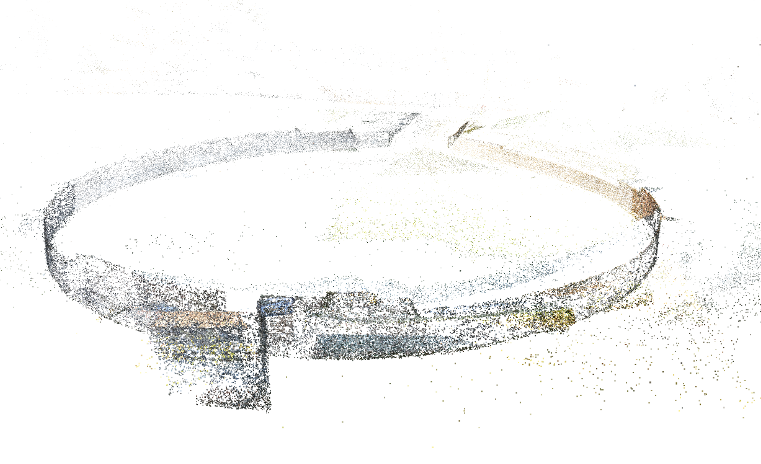
\includegraphics[width=\textwidth]{amphi_meshlab_sparse00_sm}
					\caption{Sparse Point Cloud}
					\label{amphi_sparse}
				\end{subfigure}
				\begin{subfigure}{0.5\textwidth}
					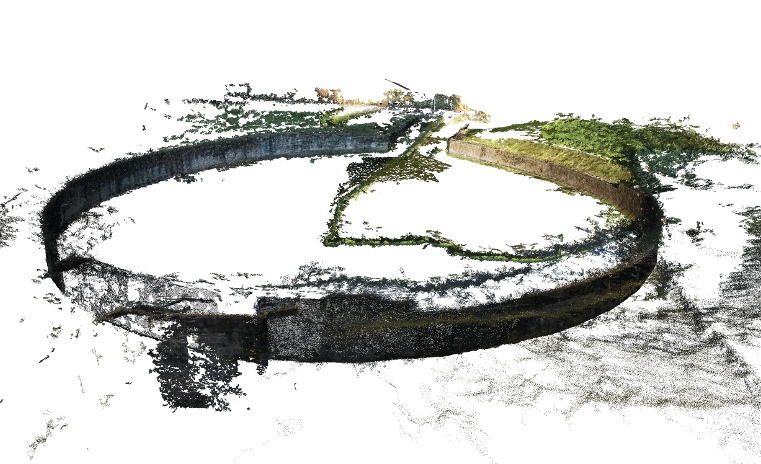
\includegraphics[width=\textwidth]{amphi_meshlab_dense00_sm}
					\caption{Dense Point Cloud}
					\label{amphi_dense}
				\end{subfigure}
				\caption{Das gallorömische Theater Engehalbinsel als sparse und dense Point Cloud}
				\label{amphi_pointclouds}
			\end{figure}			
		\subsection{Multiview Stereo} \label{mvs}
			Durch SfM ist jede Kameraposition bekannt und dadurch wie zwei Bilder zueinander stehen. Diese Information nutzt man für eine Triangulation jedes Pixels. Dadurch entsteht eine sehr dichte Point Cloud\autorefu{amphi_dense} und abhängig von den Einstellungen und der Auflösung der Fotos kann ein sehr detailreiches Modell erstellt werden.
			Dieser Schritt kann sehr lange dauern und benötigt viel Arbeitsspeicher, wenn ein detailreiches Modell erstellt werden soll.

	\section{Implementierung}  \label{imp:tech}
		Da \dronarch\ ein open source Projekt ist und auf solchen aufbaut, darf eine kurze Aufführung der verwendeten Programme und Libraries nicht fehlen.Der Source Code ist auf github verfügbar\citeu{dronarch:github}. % Mehr Details dazu in \autoref{app:imp}. 
		
		\paragraph{Python}
			Die Programmiersprache Python \citeu{python} ist wegen seiner Einfachheit und der grossen Menge an verfügbaren Libraries beliebt.
			In \dronarch\ sind alle vorbereitenden Schritte und die Koordination der einzelnen Fragmente in Python geschrieben.
			
		\paragraph{OpenCV}
			OpenCV\citeu{opencv} eine Sammlung von Computer Vision Algorithmen und bietet eine Schnittstelle für Python.
						
		\paragraph{Bundler}
			Die SfM Implementierung Bundler\citeu{bundler:homepage} von Noah Snavely wurde für die Verarbeitung einer grossen Menge an Fotos aus dem Internet geschrieben. Snavely \etal\ verwenden Bundler unter anderem dafür Monumente \citeu{Snavely:2006:PTE:1179352.1141964} oder ganze Städte \citeu{Agarwal:2011:BRD:2001269.2001293} aus Fotos aus dem Internet zu rekonstruieren.

		\paragraph{PMVS und CMVS}
			Die Kombination aus PMVS\citeu{pmvs:homepage} und CMVS\citeu{cmvs:homepage} ist für den MvS Schritt zuständig. Die Software stammt von Furukawa \etal\citeu{Furu:2010:PMVS} und wurde von ihnen für MvS mit unstrukturierten Bildern verwendet\citeu{Furu:2010}.
		